\section{Conclusion}
\label{sec:conclusion}
\par The main purpose to make a self-adaptive system for house heating system is to reduce the energy cost in the residential area. With smart heating system, it can use a big amount of energy because it will not keep heater always running and also every heater run and stop is based on the big scale space temperature not like current most heater is based on the temperature itself. By using our system, ideally the temperature and time corresponding diagram should be like the Figure \ref{fig:system_goal}. The red part of the cruel in the diagram is the heater heating process, it is quite less compared to the whole cruel in the diagram, that means that the use of the heater is quite efficient in the smart heating system.

\begin{figure}
	\centering    	
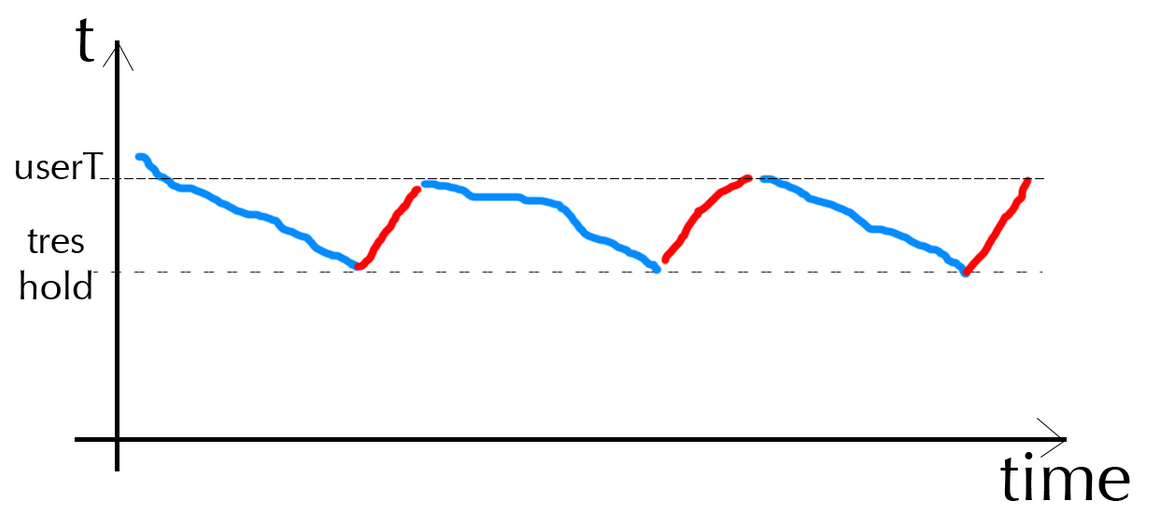
\includegraphics[width=0.90\textwidth,natwidth=610,natheight=642]{figs/system_goal.png}
  	\caption{Smart Heating System working Temperature and Time diagram}
  	\label{fig:system_goal}
\end{figure}

\par By using OSGi framework, it is quite hard to use at the beginning for us. Although the framework is based on Java, but the building process is not like normal Java application, we need to understand how the bundles work with each other and which part of the system should be service, and which part of the system should be separate bundle. These cases normally will not be considered that much in normal Java application. And also the OSGi framework has not really good IDE (Integrated Development Environment) Editors to work with, it makes our working process quite slow at the beginning when we need to set up a lot of configuration and import different bundles from external project. Although Eclipe is the IDE Editor we are using in this project, it has quite a few annoying problems. And it seems like there is no other optional IDE can be chosen in this project OSGi framework working environment. Then it makes it is quite hard to collaborate with teammates even we are using Git as version control tool because of the build path configuration and Bndtool configuration.

\par Last but no least, we believe the concept of the OSGi framework would help Java programming more efficient and more clear. And the concept of self-adaptive system is really good to work in telecommunication real-time system which is highly required for self-adaptive feature. 